\documentclass{beamer}
%\documentclass[handout]{beamer}

\usetheme{ENSIMAG}

\definecolor{redtrefle}{rgb}{0.5, 0, 0}
\definecolor{redmoka}{rgb}{0.25, 0.5, 0}
\definecolor{redminuit}{rgb}{0.5, 0, 0.5}
\definecolor{lightgray}{rgb}{0.6, 0.6, 0.6}
\definecolor{dkgreen}{rgb}{0,0.6,0}
\definecolor{gray}{rgb}{0.5,0.5,0.5}
\definecolor{mauve}{rgb}{0.58,0,0.82}
\definecolor{orange}{rgb}{1,0.45,0}
\definecolor{dkblue}{rgb}{0.098,0.098,0.44}

\usepackage[utf8]{inputenc}
\usepackage[french]{babel}
\usepackage{color}
\usepackage{verbatim}
\usepackage{graphicx}
\usepackage{listings}
\usepackage{algorithm2e}
\usepackage{empheq}

\usepackage[absolute,showboxes,overlay]{textpos}

%\TPshowboxestrue
\TPshowboxesfalse
\textblockorigin{10mm}{10mm} % origine des positions


% command to highlight text in orange
\newcommand{\alertor}[1]{\textcolor{orange}{#1}}

\usepackage{tikz}
\tikzset{visib/.style={rectangle, color=black, fill=gray!10, draw, text=black, text opacity=1, text width=#1,align=flush center}}
\tikzset{rvisib/.style={text=black,text opacity=1, text width=#1,align=flush right}}
\tikzset{invisib/.style={rectangle,color=gray,fill=gray!10,text=black,draw,text opacity=0.4, text width=#1,align=flush center}}
\newenvironment{myfancyblock}%
{\begin{center}\begin{tikzpicture}}%
{\end{tikzpicture}\end{center}}%
\newcommand{\opaqueblock}[4]{
    \node[#2=#3] (X) {#4};
}

% Settings pour l'insertion de code %
\lstset{
  language=C,
  aboveskip=3mm,
  belowskip=3mm,
  xleftmargin=9mm,
  showstringspaces=false,
  columns=flexible,
  basicstyle={\tiny\ttfamily},
  numbers=left,
  numberstyle=\tiny\ttfamily\color{mauve},
  keywordstyle=\color{orange},
  commentstyle=\color{dkblue},
  stringstyle=\color{mauve},
  breakatwhitespace=true
  tabsize=4
}

\lstset{escapechar=\§}

\title[ECC Side channel attacks]{Side Channel attacks on ECC}

\subtitle{Review of possible attacks}

\author{Franck De Goër\\Guillaume Jeanne}

\institute{SCCI - Ensimag}

\date{January, 2014}

\AtBeginSection[]
{
    \begin{frame}<beamer>
        \frametitle{Overview}
        \tableofcontents[currentsection]
    \end{frame}
}

\begin{document}

\begin{frame}
    \titlepage
\end{frame}

\begin{frame}[t]
    \frametitle{Introduction}
    \vspace{1cm}
    \begin{description}
        \item[{\bf Subjet}] Side channel attacks over ECC algorithms.
        \item[{\bf Goal}] Perform attacks to recover a secret key from a cryptoraphic algorithm using elliptic curve. \\
	Make an overview of different methods and detail some of them that have an important impact on ECC cryptography.
	
    \end{description}
\end{frame}

\begin{frame}
    \frametitle{Overview}
    \tableofcontents
\end{frame}

\begin{frame}
    \frametitle{What is a side channel attack?}
    \begin{itemize}
        \item \textcolor{black} {Take advantage of the interaction between a device and its environment.}
        \item \textcolor{black} {Apply to the embedded world: smartcards, microcontrollers}
	\item \textcolor{black} {All environement variables: time, power consumption, electromagnetic field, acoustic...}
    \end{itemize}

\end{frame}


\section{The double-and-add algorithm}
    \subsection{Universality}
    \subsection{Importance}

\section{Non-invasive attacks}

\begin{frame}
    \frametitle{Non-invasive attacks}
    \begin{itemize}
        \item \textcolor{black} {Do not destroy or alter the functioning of the device}
        \item \textcolor{black} {Cannot be detected by the owner of the device}
	\item \textcolor{black} {Physical enclosures, auditing capabilities, and attack detectors are ineffective}
	\item \textcolor{black} {$\implies$ Keys are not revoked !}
    \end{itemize}

\end{frame}

    \subsection{Timing attacks}

\begin{frame}
    \frametitle{Timing attacks}
    \begin{itemize}
        \item \textcolor{black} {First discovered side channel attack.}
        \item \textcolor{black} {Measuring the time dedicated to the computation of an algorithm .} 
	\item \textcolor{black} {Deduce how many times the program runs into a given loop.} 
	\item \textcolor{black} {Not used anymore because Power analysis is as simple and more efficient.} 
    \end{itemize}
\end{frame}


    \subsection{Power analysis}

\begin{frame}
    \frametitle{Model for processor comsuption power}
    \begin{itemize}
        \item \textcolor{black} {Each low level instruction consumes a given amount of power $p_{i}$ (depending on the number of clock cycles, registers, etc...)}
        \item \textcolor{black} {Manipulated data impact the power consumption with their hamming weight $h_{data_{i}}$.} 
    \end{itemize}
\begin{center}
    $ e_{i} = p_{i} + \sum_{j=1}^{n} \alpha_{j}. h_{data_{j,i}}$\\
\end{center} 

    $ p_{i} \approx 10^{2}.\alpha_{i}. h_{data_{i}}$\\
\end{frame}

        \subsubsection{SPA: Simple power analysis}

\begin{frame}
    \frametitle{Simple power analysis}
    \begin{itemize}
        \item \textcolor{black} {Need an oscilloscope and a card reader}
	\item \textcolor{black} {One measurement of the consumption} 
	\item \textcolor{black} {Point adding  in EC is more expensive than the point doubling} 
	\item \textcolor{black} {If the addition is computed then $d[i] = 1$}
    \end{itemize}
\end{frame}

\begin{frame}
    \frametitle{Can you recover the secret key ?}
    \begin{figure}
        \centering
        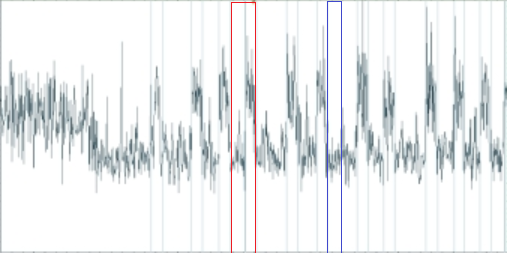
\includegraphics[scale=0.6]{img/spa.png}
        \caption{SPA against double-and-add from an IPod touch.}
    \end{figure}
\end{frame}

\begin{frame}
    \frametitle{Protection against SPA}

\end{frame}


	\subsubsection{DPA: Differential power analysis}

\begin{frame}
    \frametitle{Differential power analysis}
    \begin{itemize}
        \item \textcolor{black} {...}
    \end{itemize}
\end{frame}

\section{Perturbation attacks}
    \subsection{Model}

    \begin{frame}
        \frametitle{Fault model}
            Generally, in smart cards, we consider that we can :
            \begin{itemize}
                \item \color{black}{Inject {\tt 0x00}}
                \item \color{black}{Inject {\tt 0xFF}}
                \item \color{black}{Inject {\tt 0x??}}
            \end{itemize}
    \end{frame}

    \begin{frame}
        \frametitle{How ?}
            \begin{itemize}
                \item \color{black}{Modifiying {\tt VCC}}
            \end{itemize}
            
            \begin{figure}
                \centering
                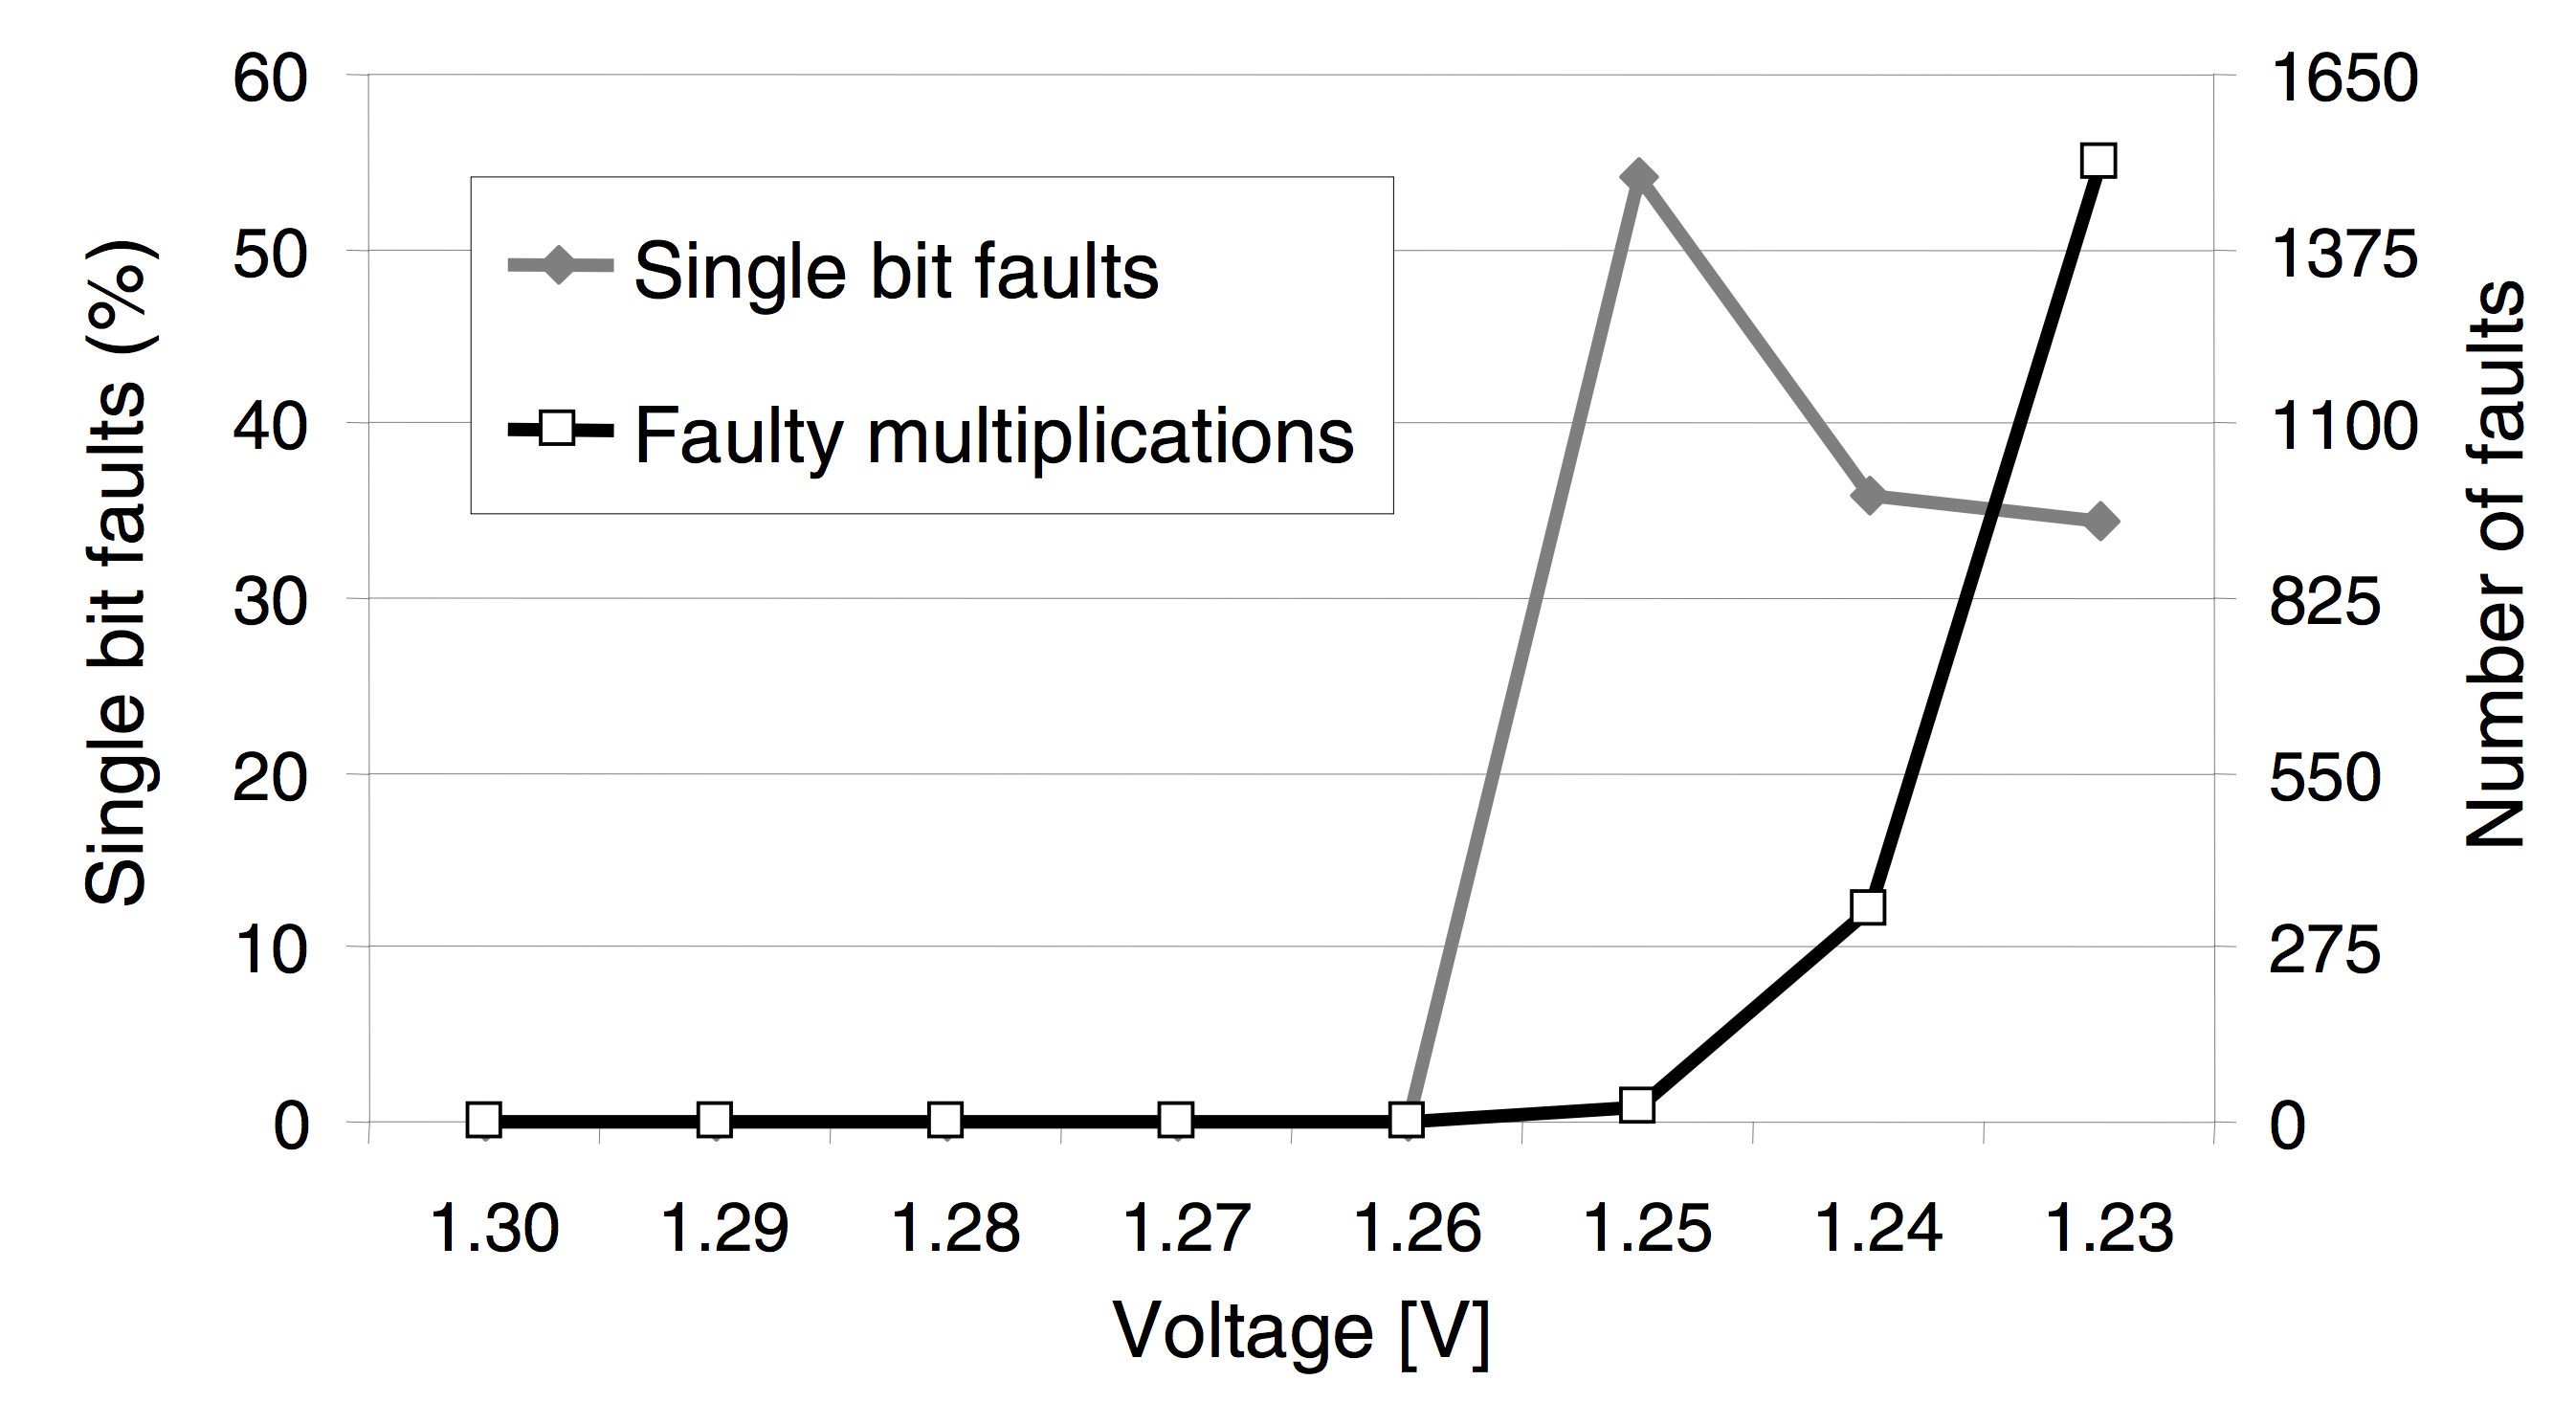
\includegraphics[width=180px]{img/power_disturbation}
            \end{figure}

    \end{frame}

    \begin{frame}
        \frametitle{How ?}
            \begin{itemize}
                \item \color{black}{Modifiying {\tt VCC}}
                \item \color{black}{With a laser}
            \end{itemize}
            
            \begin{figure}
                \centering
                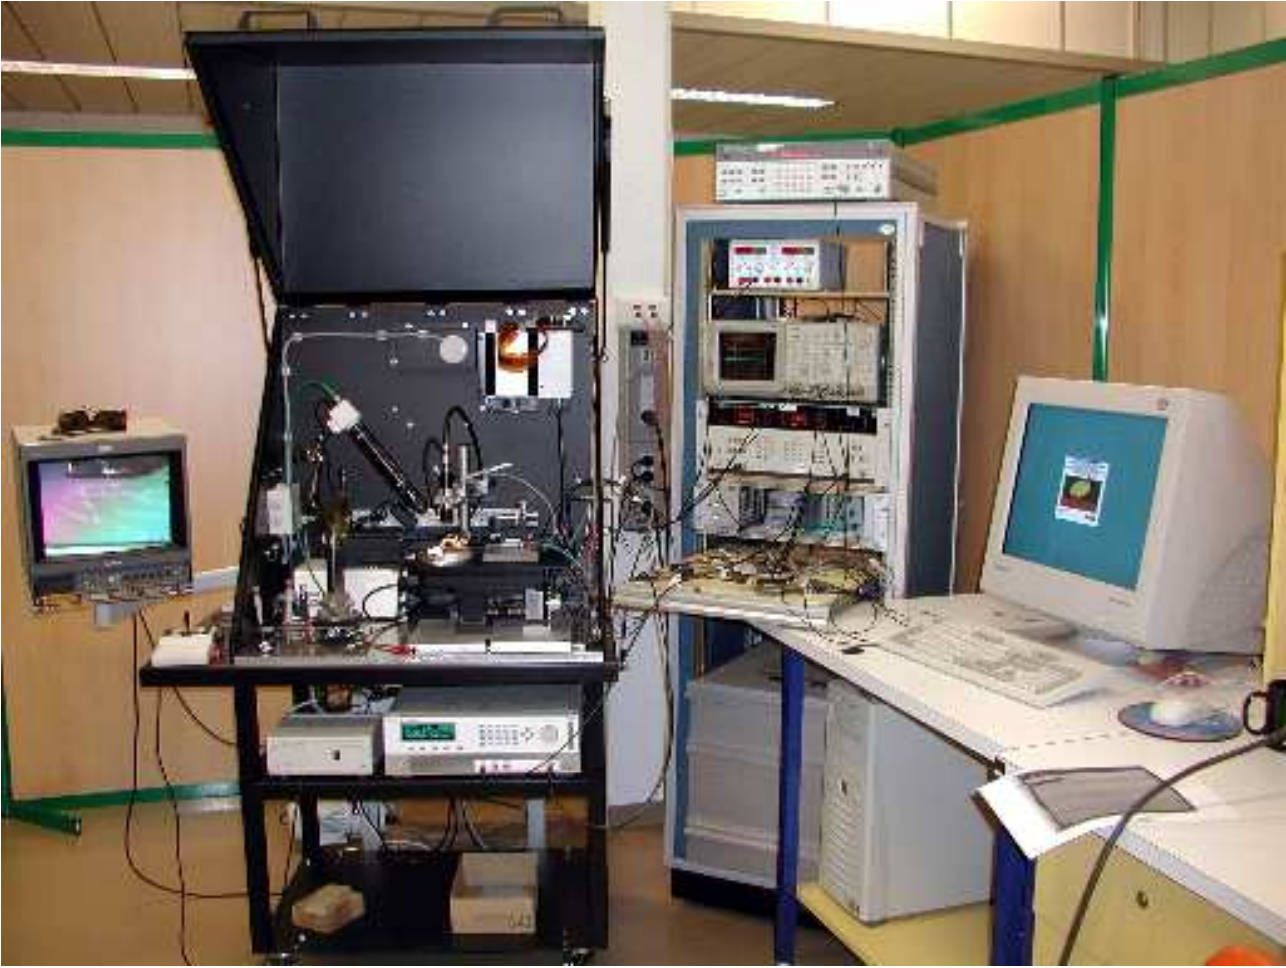
\includegraphics[width=130px]{img/laser}
            \end{figure}

    \end{frame}

    \begin{frame}
        \frametitle{In the case of the double-and-add}

            \begin{itemize}
                \item \color{black}{Modification of a register}
                \item \color{black}{$\Rightarrow$ impact on one of the coordinates}
                \item \color{black}{Bit flip}
            \end{itemize}

    \end{frame}

    \subsection{Naive attack}
    \begin{frame}
        \frametitle{First attack: malicious input}
        {\bf Idea:} Give to {\tt double-and-add} a point $P'$ that is not on the curve
    \end{frame}

    \begin{frame}
        \frametitle{Reminder: add formula}
            \label{adding-on-ec}
            $K$ a finite field, $(a_1, a_2, a_3, a_4, a_6) \in K$ \\
            $$E(K) = \{(x, y) \in K, y^2 + a_1xy + a_3y = x^3 + a_2x^2 + a_4x + a_6\} \cup \{\mathcal{O}\}$$
                    \begin{empheq}[left=\empheqlbrace]{align*}
                        x_3 &= \lambda^2 + a_1\lambda - a_2 - x_1 - x_2 \\ y_3 &= - y_1 - (x_3 - x_1)\lambda - a_1x_3 - a_3
                    \end{empheq}
                    with
                    \begin{empheq}[left=\lambda\empheqlbrace]{align*}
                        &\frac{3x_1^2 + 2a_2x_1 + a_4 - a_1y_1}{2y_1 + a_1x_1 + a_3}~if~x_1 = x_2~and~y_1 = y_2\\
                        &\frac{3x_1^2 + 2a_2x_1 + a_4 - a_1y_1}{2y_1 + a_1x_1 + a_3}~otherwise
                    \end{empheq}
    \end{frame}
    
    \begin{frame}
        \frametitle{Remarks}
            \begin{itemize} 
                \item \color{black}{Same with $P_1' \notin E(K) \Rightarrow$ result not in $E(K)$}
                \item \color{black}{Does not depend on $a_6 \Rightarrow$ possible to move to $E'(K)$}
            \end{itemize}

    \end{frame}
    
    \begin{frame}
        \frametitle{}
    \end{frame}
    
    \begin{frame}
        \frametitle{}
    \end{frame}
    
    \begin{frame}
        \frametitle{}
    \end{frame}
    
    \begin{frame}
        \frametitle{}
    \end{frame}
    
    \begin{frame}
        \frametitle{}
    \end{frame}

    \subsection{During the computation}

\begin{frame}
    \frametitle{Conclusion}

    \begin{itemize}
        \item \textcolor{black}{These attacks are efficient and not difficult to set up}
        \item \textcolor{black}{All countermeasures increase the cost of the algorithm}
	\item \textcolor{black}{Effectiveness depend on the hardware precision of the attacker}
    \end{itemize}

\end{frame}


\begin{frame}
    \frametitle{}
    \begin{center}
        {\Huge\bf\tt Thank you for your attention.}
    \end{center}
\end{frame}


%\section{Début 2}
%
%\subsection{Tout début}
%
%\begin{frame} \frametitle{Compilation de slides}
%\begin{myfancyblock}
%% First block
%\opaqueblock{1}{\textwidth}{All you have to do to initialize a GLSurfaceView is call setRenderer().
%However, if desired, you can modify the default behavior of GLSurfaceView
%by calling \alertor{one or more} of these methods before \alertor{setRenderer}:
%\begin{itemize}
%\item setDebug()
%\item setChooser()
%\item setWrapper()
%\end{itemize}
%\begin{flushright}
%(Android    2.2 API Reference)
%\end{flushright}
%}
%\invblock{2-}{\textwidth}
%
%% Second block
%\opaqueblock{2}{0.6\textwidth}{You can optionally modify the behaviour of GLSurfaceView by calling one or more debugging methods \alertor{setDebug()}, and \alertor{setWrapper()}. These methods can be called \alertor{before and or after setRender}}
%\invblock{3-}{0.6\textwidth}
%
%% Third block
%\opaqueblock{3}{0.7\textwidth}{Once the render is set, you can control whether the render draws continuously or on demand by calling \alertor{setRenderMode()}}
%
%\end{myfancyblock}
%\end{frame}

\end{document}


%%% Local Variables: 
%%% mode: latex
%%% TeX-master: t
%%% End: 
